\documentclass[a4paper]{report}

\usepackage[utf8]{inputenc}
\usepackage{geometry}
\usepackage{OldStandard}
\usepackage{microtype}
\usepackage[inline]{enumitem}
\usepackage{tabu}
\usepackage[english]{babel}
\usepackage[autostyle, english=british]{csquotes}
\MakeOuterQuote{"}

\usepackage[backend=biber,style=alphabetic,autocite=inline]{biblatex}
\addbibresource{biblio.bib}
\usepackage{makeidx}
\makeindex

\usepackage{commath}
\usepackage{amsmath}
\usepackage{amsthm}
\usepackage{amssymb}
\usepackage{mathtools}
\usepackage{mathrsfs}

\usepackage[alsoload=astro]{siunitx}

\usepackage{hyperref}

\newtheorem{thm}{Theorem}
\newtheorem{iden}[thm]{Identity}
\newtheorem{lemma}[thm]{Lemma}
\newtheorem{lem}[thm]{Lemma}
\newtheorem{prp}[thm]{Proposition}
\newtheorem{obs}[thm]{Observation}
\newtheorem{cor}[thm]{Corollary}
\newtheorem{claim}[thm]{Claim}
\newtheorem{triviality}[thm]{Triviality}
\newtheorem*{thm*}{Theorem}
\newtheorem*{iden*}{Identity}
\newtheorem*{lemma*}{Lemma}
\newtheorem*{lem*}{Lemma}
\newtheorem*{prp*}{Proposition}
\newtheorem*{obs*}{Observation}
\newtheorem*{cor*}{Corollary}
\newtheorem*{claim*}{Claim}
\newtheorem*{triviality*}{Triviality}
\theoremstyle{definition}
\newtheorem{defn}[thm]{Definition}
\newtheorem{ex}[thm]{Example}
\newtheorem{exs}[thm]{Examples}
\newtheorem{con}[thm]{Construction}
\newtheorem{axs}[thm]{Axioms}
\newtheorem{ax}[thm]{Axiom}
\newtheorem{alg}[thm]{Algorithm}
\newtheorem{exercise}[thm]{Exercise}
\newtheorem{rem}[thm]{Remark}
\newtheorem*{defn*}{Definition}
\newtheorem*{ex*}{Example}
\newtheorem*{con*}{Construction}
\newtheorem*{alg*}{Algorithm}
\newtheorem*{exercise*}{Exercise}
\newtheorem*{rem*}{Remark}

\usepackage[notextcomp]{stix}
\newcommand{\df}[1]{\textbf{#1}\index{#1}}
\newcommand{\ray}{\overrightarrow}
\renewcommand\qedsymbol{$\vrectangleblack$}

\title{Topics in Geometry}
\author{Alex Elzenaar}
\date{\today}

\begin{document}
  \maketitle

  \clearpage
  \thispagestyle{plain}
  \par\vspace*{.35\textheight}{\centering\itshape In another moment Alice was through the glass and had jumped lightly down into the Looking-glass room... Then she began looking about, and noticed that what could be seen from the old room was quite common and uninteresting, but that all the rest was as different as possible. \autocite[127]{carroll} \par}

  \tableofcontents

  \clearpage
  \addcontentsline{toc}{chapter}{Preface}
  \chapter*{Preface}
  These notes, which I wrote in 2019, are intended to be an introduction to geometry for younger students who have not learned the subject
  before. I hope that I have included a good balance of practical numeracy material (on measurement, and trigonometry), traditional Euclidean geometry,
  and some more modern topics (isometries and symmetries being the `core' of this discussion).

  The notes are structured as a series of loosely connected exercises, many of which require mathematical justification; I have consciously
  decided not to follow a purely axiomatic approach in the style of Euclid, but I think enough of the structure has been erected to allow
  an axiomatic study to be motivated by --- or at the very least not precluded by --- the material within. One good modern axiomatic treatment
  is given in \autocite{lee}.

  There are not many diagrams in these notes; this is by design, as I feel that any diagrams which I provide would be far inferior in terms of actual
  learning content than diagrams drawn by students themselves. The formatting of these notes, with a far wider margin than even \LaTeX{} normally
  includes, is designed with copious note-taking in mind.

  Needless to say, these notes are wholly and fundamentally unusable as self-study material at Y11. I would recommend a book like \autocite{lang}
  or \autocite{birkhoff} for this purpose.

  There is more material here than can reasonably be covered in the ten weeks or so that schools tend to spend on geometry; my intent is
  that the instructor picks and chooses material beyond the core material, and my hope is that students find it sufficiently interesting
  to continue glancing at the notes for their own amusement.

  I also wish to note that a large proportion of these notes overlaps in content with my Level 2 notes and my Level 3 geometry notes; this is
  mainly because I usually feel the need to include a lot of extra content in higher level notes that would be better placed here.

  \section*{Recommendations for suplementary and further reading}
  References are given throughout the notes when something of particular historical or mathematical interest is discussed; however, many
  of the references are intended more for the teacher than for the student. I would like to take this opportunity to highlight a few of
  my favourites.

  If one is interested in classical geometry, then books like \autocite{sved} or \autocite{coxeterRevisited} are highly recommended.
  For more modern geometry, especially for students who have the basics of calculus available, \autocite{coxeterIntro} is a classic.
  There are a variety of problem books available: one such book is \autocite{challenging}, though there are many others.

  The author's favourite geometry book, however, is \autocite{berger}.

  \newgeometry{left=2cm,right=8cm}
  \setcounter{chapter}{-1}
  \chapter{Proof in mathematics}
  \begin{center}
    \begin{minipage}{0.7\textwidth}\itshape
      A mathematician does not want to be told something: they want to find it out for themself. \autocite[19]{sawyerPrelude}
    \end{minipage}
  \end{center}
  In this topic, we are going to prove things. This is a simple statement, but one it is worth spending a bit of time
  thinking about.

  First of all, what is \df{mathematical proof}? The most simple definition is that a proof is an explanation of why a
  statement is true. More precisely, one starts from a set of accepted assumptions (the \df{hypotheses} of the proof), and one argues
  why certain conclusions \emph{must} be true.

  Proof is what sets mathematics apart from the sciences --- in physics and chemistry, for example, one does not prove
  things simply by thought (a physical theory is incorrect if it disagrees with experiment, no matter how logically
  sound it is). In all fields of mathematics, things must be proved before they are used.

  Here are some more words:
  \begin{itemize}
    \item A \df{theorem} is a true statement that has been deduced (via a mathematical proof) from
          some agreed assumptions. (For example, Pythagoras' theorem.)
    \item A \df{proposition} is a small theorem.
    \item An \df{axiom} or \df{postulate} is a basic assumption that is accepted without proof. (For example, `all right
          angles are equal'.)
  \end{itemize}

  \chapter{Basic theory}
  The first known systematic treatment of geometry is Euclid's \emph{Elements} (one particularly nice
  edition is \autocite{euclid}). Euclid lived in Alexandria (in Greek Egypt) in around 300 BCE; his
  book is the oldest known treatment of a field of mathematics in a deductive way, that is by starting
  with a small set of `obvious' (i.e. unproved) statements with the goal of deducing as much theory
  as possible using purely logical reasoning.

  Euclid's development of geometry is rather lacking in a few ways, at least if it is judged against
  modern mathematical standards; however, the results proved by Euclid still form the basic foundation
  of the geometry which we will be studying here. For a commentary on Euclid from a mathematical perspective,
  see \autocite{hartshorne}.

  Rather than work axiomatically, we will take for granted that the things we discuss
  are well-defined and exist, and we will allow ourselves to think of the foundations of
  geometry in an intuitive fashion rather than a precise fashion. For a precise, axiomatic
  development of the foundations of geometry see \autocite{lee}.

  \section{Terminology}
  We will take our \df{space} to be a set of \df{points}, which we will label with
  capital Roman letters $ A $, $ B $, $ C $, and so on. Through every pair of points
  we will be allowed to draw a unique \df{line}; the line through $ A $ and $ B $ will be
  denoted by $ \overline{AB} $. The portion of the line that lies \emph{between} $ A $
  and $ B $ will be called a \df{segment} and will be denoted by $ [A,B] $. To
  each segment we assign a number, called the \df{length} of the segment $ [A,B] $
  or the \df{distance} between $ A $ and $ B $, in the usual way (i.e. the length is `whatever
  the ruler reads when you hold it up to the segment'). The length of $ [A,B] $ will be denoted by $ \abs{AB} $.

  \begin{prp}
    If $ \ell $ and $ m $ are distinct lines (we will use lowercase Roman letters to denote lines), then $ \ell $ and $ m $
    either do not intersect or intersect at precicely one point. There are no other options.
  \end{prp}
  \begin{proof}
    Suppose $ \ell $ and $ m $ intersect at more than one point: say they intersect at two different points, $ A $ and $ B $. We
    need to show that $ \ell $ and $ m $ cannot be distinct lines. But by our assumption above, there is a \emph{unique} line between any
    two points; hence $ \ell $ and $ m $ must both be this unique line, and must therefore be the same.
  \end{proof}

  Let $ \ell $ and $ m $ be lines.  Then $ \ell $ and $ m $ are said to be \df{parallel} if they do not intersect in exactly one point; by
  the above proposition, this means that they must intersect either zero times or they must be the same line. If $ \ell $ and $ m $ are
  parallel, we will write $ \ell \parallel m $.

  It is necessary for us to assume one thing about parallel lines without proof:

  \begin{ax}[Parallel postulate]\index{Parallel postulate}
    If $ \ell $ is a line, and $ P $ is any point that does not lie on $ \ell $, then there is a unique line through $ P $
    parallel to $ \ell $.
  \end{ax}

  This postulate was Euclid's fifth axiom, and is of a much more sophisticated nature than the other four (which stated
  things like `it is possible to draw a unique line through two points' and `all right angles are equal'); it was thought
  for over a thousand years that this postulate was so much more complex than the others that it must follow from them
  as a theorem. A later commentator, Proclus, wrote in fifth century Athens that ``[the parallel postulate] ought to be
  struck from the postulates altogether. For it is a theorem --- one that invites many questions, which Ptolemy proposed
  to resolve in one of his books --- and requires for its demonstration a number of definitions as well as theorems''
  (quoted in \autocite[296-297]{hartshorne}).

  It turns out that proving the parallel postulate from Euclid's other four axioms is impossible, for a fairly simple reason:
  it is possible to exhibit a perfectly reasonable geometry that satisfies the first four but not the fifth. The most familiar example is a
  sphere. Dix a line of latitude and a point not on that line. Then all the lines through that point intersect
  the original line, so there are no parallel lines!

  \begin{exercise}
    Show that, if $ \ell $ and $ m $ are lines, then:
    \begin{enumerate}
      \item $ \ell \parallel \ell $;
      \item if $ \ell \parallel m $ then $ m \parallel \ell $;
      \item if $ \ell \parallel m $ and $ m \parallel n $ then $ \ell \parallel n $ (where $ n $ is another line).
    \end{enumerate}
    We say that being parallel is an \df{equivalence relation}.
  \end{exercise}

  \begin{exercise}
    Suppose $ \ell $ and $ m $ are parallel; let $ n $ be a line, and suppose it intersects line $ m $ at a point $ P $. How
    are lines $ \ell $ and $ n $ related?
  \end{exercise}

  A \df{polygon}, or more specifically an \df{$ n$--gon} where $ n $ is some number, is a set of points $ A_1, A_2, ..., A_n $ (all different)
  together with the line segments $ [A_1, A_2] $, $[A_2, A_3]$, ..., $[A_n, A_1] $. The polygon will be denoted by $ A_1A_2A_3\cdots A_n $. The
  points defining the polygon are called the \df{vertices}, and the line segments are called the \df{edges} of the polygon. Two polygons
  are called \df{equal} if they share the same points and edges, up to relabelling. Note that we allow edges to cross each other; note also that
  the order of the points matters: $ ABCD $ is not the same polygon as $ ACBD $.

  A polygon with three edges is called a \df{triangle}; a polygon with four edges is called a \df{quadrilateral} or a \df{quadrangle}. If
  all the sides of a polygon are the same length, it is called \df{equilateral}.

  \begin{exercise}
    Let $ A $, $ B $, $ C $, and $ D $ be pairwise distinct points (i.e. no two are the same); how many different 4-gons
    can you form with these points as vertices?
  \end{exercise}

  The \df{circle} with \df{centre} $ O $ and \df{radius} $ r $, where $ O $ is a point and $ r $ is a positive number,
  is the set of all points that lie at a distance $ r $ from $ O $ (i.e. a point $ X $ lies on the circle precisely
  when $ \abs{OX} = r $).

  \begin{exercise}
    Let $ [A,B] $ be a line segment. Draw the circle with centre at $ A $ of radius $ \abs{AB} $, and the circle with centre $ B $
    of radius $ \abs{AB} $. These two circles will intersect at two points, $ X $ and $ Y $. What kinds of triangles are $ ABX $ and $ ABY $?
  \end{exercise}

  \begin{exercise}
    Let $ [A,B] $ be a line segment. The \df{midpoint} of $ [A,B] $ is the point $ M $ such that $ \abs{AM} = \abs{BM} $. Can you
    find $ M $ by drawing only circles of a given centre and radius?
  \end{exercise}

  \section{Angles}
  Let $ O $, $ A $, and $ B $ be three distinct points. A line eminating from $ O $ and passing through $ A $ indefinitely will be called the \df{ray} $ \ray{OA} $;
  if we consider the two rays $ \ray{OA} $ and $ \ray{OB} $ then together they split up the space into two regions, called the \df{angles} associated with
  the rays. The angle $ \angle AOB $ is the angle which is found by starting at $ \ray{OA} $, and then rotating anticlockwise to $ \ray{OB} $. In other words,
  the notation `walks' from $ A $, to $ O $, and to $ B $, and we take the region on our left. The angle $ \angle BOA $ is the angle found by starting at $ B $,
  walking to $ A $, and taking the region on our left. In all these cases, $ O $ is called the \df{vertex} of the angle.

  If $ A $ and $ B $ are the same point, then we still say that $ AOB $ is an angle; however, we will determine from context in each case
  whether we mean the angle with no interior or the angle whose interior is the entire space.

  If $ \angle AOB $ is an angle, we may draw a circle at $ O $; then the portion of the circle lying within each region is called an \df{arc} of
  the circle, and the portion of the inside of the circle is called a \df{sector} of the circle.

  There are several different ways of assigning a measure to angles; we will use the so-called \df{degree} measure here. The idea is to
  associate with a full angle --- that is, an angle $ \angle OAB $ such that a circle at $ O $ has no arc cut off --- a measure of \ang{360}.

  If $ A $, $ O $, and $ B $ all lie on a line (if they are \df{colinear}), we will call the angle $ \angle AOB $ the \df{straight angle};
  it is clear that any circle around $ O $ is divided into two equal parts, and so the angle $ \angle OAB $ must have measure of one-half
  a full turn; that is, \ang{180}. An angle whose measure is one-half a straight angle is called a \df{right angle}, and has measure \ang{90}.

  We occasionally split a degree into sixty \df{minutes}, and one minute into sixty \df{seconds}; the notation \ang{30;40;2} represents
  an angle with measure 30 degrees, 40 minutes, and 2 seconds (i.e. $ 30 + \frac{40}{60} + \frac{2}{60 \times 60} \approx \ang{30.6672} $);
  this notation is really only used in navigation in the modern world, and you will hardly ever see it.

  Angles that are measured anticlockwise are positive; angles that are measured clockwise are negative. Two angles are said to be \df{congruent}
  (we will often be flexible with language and call them equal) if they have the same measure.

  \begin{exercise}
    An angle \ang{15} cuts out an arc $ a $ on a circle whose circumference is \SI{5}{\centi\metre}. How long is the arc $ a $?

    Use a protractor to draw a picture and check.
  \end{exercise}

  \begin{exercise}
    Wellington is around \ang{41.3} south of the Equator. The circumference of the earth is around \SI{40000}{\kilo\metre}. How far
    away, around the Earth, is Wellington from the nearest point on the Equator?
  \end{exercise}

  Two angles who share a common vertex are called \df{adjacent}. If $ \angle{AOB} $ and $ \angle{BOC} $ are adjacent,
  then $ \angle{AOC} = \angle{AOB} + \angle{BOC} $.

  The following terms are standard, but basically unimportant. We will not use them in these notes, but
  they are included for reference purposes.
  \begin{enumerate}
    \item Two angles whose measure sum to \ang{180} are called \df{supplementary}.
    \item Two angles whose measure sum to \ang{90} are called \df{complementary}.
    \item If an angle has measure less than a right angle it is called \df{acute}.
    \item If an angle has measure greater than a right angle but less than a straight angle it is called \df{obtuse}.
    \item If an angle has measure greater than a straight angle it is called \df{reflex}.
  \end{enumerate}

  Suppose two distinct lines intersect at a point $ O $. Then these lines define four angles; suppose their measures are, clockwise, $ \alpha $,
  $ \beta $, $ \gamma $, and $ \delta $ (we will always use Greek letters to denote angles). Then each pair of non-adjacent
  angles ($ \alpha $ and $ \gamma $, and $ \beta $ and $ \delta $) is called a pair of \df{opposite} angles.

  \begin{exercise}
    Suppose $ \alpha $, $ \beta $, $ \gamma $, and $ \delta $ are measures of angles organised in this way; show that $ \alpha = \gamma $, and $ \beta = \delta $.
    (In other words, opposite angles have equal measure.)
  \end{exercise}

  \begin{exercise}
    Suppose $ \ell $ and $ m $ intersect at a point $ X $, and one of the angles between the lines at $ X $ is a right angle. Show that
    all four are right angles.

    Such lines are called \df{perpendicular}, and we write $ \ell \perp m $.

    If two lines are parallel, and a third line is perpendicular to one of them, then it is perpendicular to both.
  \end{exercise}


  \begin{exercise}
    Let $ \ell $ and $ m $ be parallel lines, and suppose $ n $ is a third line which intersects them at $ A $ and
    $ B $ respectively. What are the relationships between the angles around $ A $ and the angles around $ B $?

    Suppose it is not known that $ \ell $ and $ m $ are parallel. Could you use knowledge of the angles around $ A $
    and $ B $ to check whether they are?
  \end{exercise}

  \begin{exercise}
    Let $ [A,B] $ be a segment. The unique line $ \ell $ that passes through the midpoint of $ [A,B] $ and is perpendicular to $ \overline{AB} $
    is called the \df{perpendicular bisector} of $ [A,B] $.

    Given such a segment, can you draw the perpendicular bisector using only a compass and a straightedge --- i.e. without a protractor?
  \end{exercise}

  If $ A_1A_2A_3\cdots A_n $ is a polygon such that no edges cross (we will call such polygons \df{normal}), then to each vertex
  we may assign two angles. Draw a small circle around each vertex that doesn't include any other vertex; then the arc of the circle
  that lies inside the polygon is cut off by one of the angles at the vertex whose rays include the edges of the polygon, and this
  angle is called the \df{interior angle} of the polygon. The other angle is called the \df{exterior angle}. If a polygon's interior
  angles are all acute, then the polygon is called \df{convex}. If all the interior angles of a polygon are equal, the polygon is
  called \df{equiangular}. If a polygon is both equiangular and equilateral, it is called \df{regular}.

  \begin{exercise}
    The internal angles of a triangle add to \ang{180}. The internal angles of a normal quadrilateral add to \ang{360}. What do the internal
    angles of a normal $ n$-gon add to?
  \end{exercise}

  \begin{exercise}\label{ex:typesofquadrilaterals}
    Draw examples of all the following.

    A regular quadrilateral is usually called a \df{square}. By the previous exercise, the internal angles of a square are all $ \ang{360}/4 = \ang{90} $.
    A quadrilateral such that all internal angles are right angles is called a \df{rectangle}. A non-equiangular but equilateral quadrilateral
    is called a \df{rhombus}. A quadrilateral such that both pairs of opposite sides are parallel is called a \df{parallelogram}. A quadrilateral
    such that at least one pair of opposite sides is parallel is called a \df{trapezoid}.
  \end{exercise}

  A \df{chord} of a circle is a line segment with endpoints on the circle. A \df{diameter} is a chord passing through the centre.

  \begin{exercise}[Inscribed angle theorem]
    Draw a circle with centre $ O $; let $ AB $ be a chord of the circle, and pick a point $ X $ on the circle.
    Then the measure of $ \angle AOB $ is twice the measure of $ \angle {AXB} $. What if $ X $ is (a) inside, (b) outside the circle?
  \end{exercise}

  \begin{exercise}[Thale's theorem]
    Draw a circle with centre $ O $; let $ AB $ be a diameter of the circle, and pick a point $ X $ on the circle.
    Then $ AXB $ is a right-angled triangle with right angle at $ X $.
  \end{exercise}

  \section{Congruence and similarity}
  Suppose $ \mathscr{F} $ and $ \mathscr{G} $ are \df{figures} (complicated collections of points, like polygons or circles). It is
  fairly intuitive that if we can `lift one up, and put it down exactly on the other one', then the two figures are the same shape and size.
  We would like to make this more precise.

  \begin{defn}
    An \df{isometry} $ \mathsf{Isom} $ is a \df{transformation} -- a way of moving every point $ X $ in our space to another point $ \mathsf{Isom}(X) $ ---
    such that whenever $ X $ and $ Y $ are points, the distance $ \abs{\mathsf{Isom}(X) \mathsf{Isom}(Y)} $ is equal to the distance $ \abs{XY} $.
  \end{defn}

  A point which is not moved by a transformation is called a \df{fixed point}.

  It is non-trivial to prove the following theorem, within which we will intermix some definitions.
  \begin{thm}[Classification of plane isometries]\label{thm:classisom}
    There are precisely five kinds of isometry.
    \begin{enumerate}
      \item The \df{identity transformation} $ \mathsf{Id} $, which leaves everything where it is. (In other words, every point is a fixed point.)
      \item The \df{translations} $ \mathsf{Tr}_{XY} $ (one for each pair of distinct points $ X $ and $ Y $) which send every point in the plane
            to the point a distance $ \abs{XY} $ away, in the direction parallel to $ \ray{XY} $. (No points are fixed.)
      \item The \df{rotations} $ \mathsf{Rot}_{O,\theta} $ (one for each point $ O $ and angle $ \theta $ between, but not including, zero and a
            full turn), which send every point $ X $ on the circle centred at $ O $ passing through $ X $ to the unique point $ Y $ such
            that $ \angle XOY $ has measure $ \theta $. (The point $ O $ is fixed, and no others.)
      \item The \df{reflections} $ \mathsf{Ref}_\ell $ (one for each line $ \ell $), which send every point $ X $ to the unique point $ X' $ such that
            $ \ell $ is the perpendicular bisector of $ XX' $. (The line $ \ell $ is fixed and no other points are; every line perpendicular to $ \ell $
            is transformed to itself, but no other lines except $ \ell $ are.)
      \item The \df{glide reflections} $ \mathsf{GlRef}_{\ell, x} $ which consist of a reflection across $ \ell $ and then a translation along $ \ell $
            through a distance $ x $. (The line $ \ell $ is fixed, and no other points are fixed, and no other lines are transformed to themselves.)
    \end{enumerate}
    Further, every transformation is uniquely determined by which points and lines it fixes (i.e. transforms onto themselves).
  \end{thm}
  \begin{proof}
    See: \autocite[chapter 5]{artin}, or \autocite[chapter 3]{coxeterIntro}. We will consider isometries in more detail later on.
  \end{proof}

  If we do one isometry after another, the total is still an isometry. Further, the action of undoing an isometry is also an
  isometry. (Isometries are said to form a \df{group}.)

  \begin{exercise}\leavevmode
    \begin{enumerate}
      \item Two successive rotations around different points form a translation.
      \item Two successive reflections across lines which intersect at exactly one point form a single rotation about that point.
      \item Two successive reflections across lines which do not intersect form a translation.
      \item Two successive reflections across the same line form the identity.
    \end{enumerate}
  \end{exercise}

  Two figures $ \mathscr{F} $ and $ \mathscr{G} $ are called \df{congruent} if there is an isometry that maps
  one onto the other: more precisely, $ \mathscr{F} \cong \mathscr{G} $ if and only if there is an isometry $ \mathsf{Isom} $
  such that whenever $ X $ is a point on $ \mathscr{F} $ then $ \mathsf{Isom}(X) $ is a point on $ \mathscr{G} $, and
  whenever $ Y $ is a point on $ \mathscr{G} $ then there is a point $ X $ on $ \mathscr{F} $ such that $ \mathsf{Isom}(X) = Y $.
  (In other words, if $ \mathsf{Isom} $ is a one-to-one correspondence between the two figures.)

  \begin{exercise}
    Convince yourself (no rigorous proof necessary, but \emph{convince yourself}) that two triangles are congruent
    precisely when they have equal edge lengths.
  \end{exercise}

  It is possible that two figures can be the same shape even if they are not the same size. For example, all
  circles centred at a given point can be transformed into each other by shrinking and stretching equally in
  all directions.

  \begin{defn}
    A \df{dilation} $ \mathsf{Dil}_{O,\mu} $ is a transformation that sends each point $ X $ to the point on the ray $ \ray{OX} $
    that is a distance $ \mu \abs{OX} $ from $ O $.

    Two figures $ \mathscr{F} $ and $ \mathscr{G} $ are said to be \df{similar}, and we write $ \mathscr{F}\sim\mathscr{G} $,
    if one can be transformed onto the other by means of a succession of dilations and isometries (i.e. rigid movements and
    shrinking and stretching equally in all directions.)
  \end{defn}

  \begin{exercise}\leavevmode
    \begin{enumerate}
      \item All circles are similar.
      \item Two rectangles, of side lengths $ x_1 $ and $ y_1 $ and $ x_2 $ and $ y_2 $ respectively, are similar
            when $ x_1/x_2 = y_1/y_2 $.
    \end{enumerate}
  \end{exercise}

  There are a number of useful characterisations of similar triangles.

  \begin{prp}\label{ex:similar}
    Two triangles $ ABC $ and $ DEF $ are similar if one of the following is true (and therefore all are true):
    \begin{enumerate}
      \item The following relationship holds:
        \begin{equation}\label{eqn:trisimilar}
          \frac{\abs{AB}}{\abs{DE}} = \frac{\abs{BC}}{\abs{EF}} = \frac{\abs{CA}}{\abs{FD}} ~(= \mu)
        \end{equation}
      \item The angles at $ A $ and $ D $ are congruent, and $ \frac{\abs{AB}}{\abs{DE}} = \frac{\abs{CA}}{\abs{FD}} ~( = \mu)$.
      \item There is a matching between two vertices of the two triangles such that matched vertices have congruent angles.
      \item There is a matching between all three vertices of the two triangles such that matched vertices have congruent angles.
    \end{enumerate}
  \end{prp}
  \begin{proof}
    See \autocite[chapter 12]{lee}.
  \end{proof}

  \begin{exercise}
    Let $ ABC $ be a triangle. Show that the following are equivalent (i.e. if one is true then the other is true):
    \begin{enumerate}
      \item The interior angles at $ B $ and $ C $ are congruent.
      \item The lengths $ \abs{AB} $ and $ \abs{AC} $ are equal.
    \end{enumerate}
    If one (and therefore both) hold, then $ ABC $ is called \df{isosceles}.
  \end{exercise}

  \section{Perimeter and circumference}
  The \df{perimeter} of a polygon $ \mathscr{F} = A_1 A_2 \cdots A_n $ is defined to be the sum
  \begin{equation}
    \mathcal{P}(\mathscr{F}) = \abs{A_1 A_2} + \abs{A_2 A_3} + \cdots + \abs{A_{n - 1} A_n} + \abs{A_n A_1}.
  \end{equation}

  \begin{exercise}\label{ex:circumference}
    Let $ \mathscr{c} $ be a circle, with centre $ O $ and radius $ r $. Pick $ n $ points equally spaced
    about the circumference of the circle, $ A_1,...,A_n $; so $ A_1\cdots A_n $ is a regular $ n$--gon.
    It is clear that, as $ n $ increases, the perimeter of the $ n$--gon approaches the circumference
    of the circle. Call this perimeter $ p_n $.

    Let $ \mathscr{C} $ be a second circle centred at $ O $ (two circles are \df{concentric} --- i.e. they
    have the same centre); let $ A_1' $ be the point of intersection between $ \ray{OA_1} $ and $ \mathscr{C} $, $ A_2' $ the
    point of intersection between $ \ray{OA_2} $ and $ \mathscr{C} $, and so forth. Call the perimeter of the resulting
    regular $ n$--gon $ P_n $.

    \begin{enumerate}
      \item Show that $ OA_1A_2 $ is similar to $ O A_1' A_2' $.

      \item Use this to show for every $ n $, $ \frac{P_n}{R} = \frac{p_n}{r} $.

      \item Since this holds for all $ n $, we can conclude that if $ P $ is the circumference of
            $ \mathscr{C} $ and $ p $ is the circumference of $ \mathscr{c} $, $ P/R = p/r $. Hence
            show that the ratio of circumference to radius is the same for every circle.
    \end{enumerate}
  \end{exercise}

  For historical reasons, the number $ \pi $ is defined to be one-half of this ratio: $ \pi = P/2R $. It
  turns out that
  \begin{equation}
    \pi = 3.14159265358979323846264338327950...
  \end{equation}

  We have now got a formula for the circumference of a circle of radius $ r $:
  \begin{equation}
    C = 2\pi r.
  \end{equation}

  \begin{exercise}\label{ex:piupperbound}
    We can exploit a fact about perimeters to show that $ \pi < 4 $.
    \begin{enumerate}
      \item What is the circumference of a circle with diameter 1?
      \item Draw the square with side-edge 1 that just touches this circle at the centre of each
            of its sides. What is the perimeter of this square?
      \item Using your picture, how are the two perimeters related? Hence show that $ \pi < 4 $.
      \item How could you improve your upper estimate of $ \pi $?
    \end{enumerate}
    In the next section we will show that $ \pi > 2 $ (exercise \ref{ex:pilowerbound}).
  \end{exercise}

  \section{Area}
  The \df{area} of a square $ \mathscr{S} $ of side length $ x $ is defined to be $ \mathcal{A}(\mathscr{S}) = x^2 $.

  We will now extend the idea of area to more complicated figures; the basic ideas we want are the following:
  \begin{axs}[Area function]
    Suppose we define some way of assigning a number to a collection of different figures (for example, we have just assigned a
    number --- area --- to every figure in the collection of squares). We will say that this method of assigning numbers is a \df{Jordan
    area method} if the following are true:
    \begin{enumerate}
      \item Every figure in our collection is assigned a number which is zero or positive.
      \item If we assign a number to two figures, one of which lies inside the other, the inside figure has a smaller number.
      \item If we can split up a figure $ \mathscr{F} $ into a finite number of non-overlapping figures $ \mathscr{F}_1, ..., \mathscr{F}_n $
            which are in our collection, then the figure $ \mathscr{F} $ is in our collection and we assign to it the sum of the
            numbers we assigned to $ \mathscr{F}_1, ..., \mathscr{F}_n $.
      \item The method assigns to every square $ \mathscr{S} $ the number $ \mathcal{A}(\mathscr{S}) $ as already established.
      \item The method assigns to every figure with no inside (e.g. a line, or a collection of lines, or a single point,...) the number 0.
      \item If $ \mathscr{F} \cong \mathscr{G} $, then the numbers assigned to $ \mathscr{F} $ and $ \mathscr{G} $ are equal.
    \end{enumerate}
  \end{axs}
  It turns out that there is only one way of assigning area to all the things we are used to which satisfies these properties in a nice
  way (we do need to phrase them more precisely to prove this, and we won't do it here. See \autocite[chapter 8]{lands}, or \autocite[chapter 5]{hartshorne}.)
  The basic idea is that we take all the figures we're interested in measuring, we fit into them lots of little squares, and then we add up the areas of the
  little squares. We will now have a look at this kind of technique in a superficial way that is, nonetheless, rather convincing; in fact, the methods
  we use here were those used by the Greeks.

  \begin{exercise}
    Let $ ABCD $ be a rectangle, such that $ \abs{AB} = \abs{CD} = x $ and $ \abs{BC} = \abs{DA} = y $. Show that $ \mathcal{A}(ABCD) = xy $.
  \end{exercise}
  \begin{exercise}
    Let $ ABC $ be a triangle such that $ \abs{BC} = b $. Let $ A' $ be the point on $ \overline{BC} $ such that $ \overline{AA'} \perp \overline{BC} $;
    let $ \abs{AA'} = h $. (The line $ \overline{AA'} $ is called an \df{altitude} of the triangle.) Show that $ \mathcal{A}(ABC) = \frac{1}{2}bh $.
  \end{exercise}

  \begin{exercise}
    In order to represent a piece of large land on a small flat map, we shrink every length equally according to a given ratio. We say
    a map is given to a scale of 1:\num{1000} if one unit of measurement on the map represents 1000 such units in the real world. (So
    a length of 1 metre on the map would represent an actual length of 1 kilometre.)
    \begin{enumerate}
      \item The plan of a plot of land has the shape of a square with side length \SI{10.0}{\centi\metre}. If the plan
            is to a scale of 1:\num{10000}, what is the area and perimeter of the plot of land?
      \item The following figure (\autocite[21]{kutepov}) presents the plan of a plot of land drawn to a scale of 1:\num{1000}.
            If $ \abs{AC} = \SI{6}{\centi\metre} $, $ \abs{AD} = \SI{7.6}{\centi\metre} $, $ h_1 = \SI{3}{\centi\metre} $, $ h_2 = \SI{4.8}{\centi\metre} $,
            and $ h_3 = \SI{3.2}{\centi\metre} $, compute the area of the plot.
            \begin{center}
              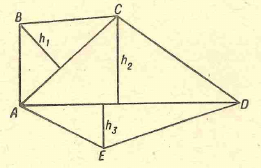
\includegraphics[width=0.5\textwidth]{landplot}
            \end{center}
      \item On the extracts from the LINZ maps below, the side length of a square is \SI{1}{\kilo\metre}. Calculate the area of (a) Somes Island,
            and (b) each of the Twin Lakes (the Macaskill Lakes).
            \begin{center}
              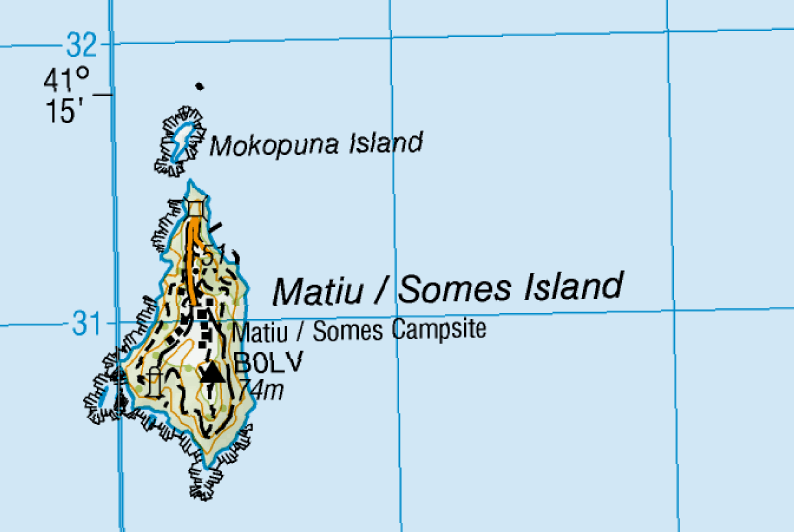
\includegraphics[width=0.45\textwidth]{somes}~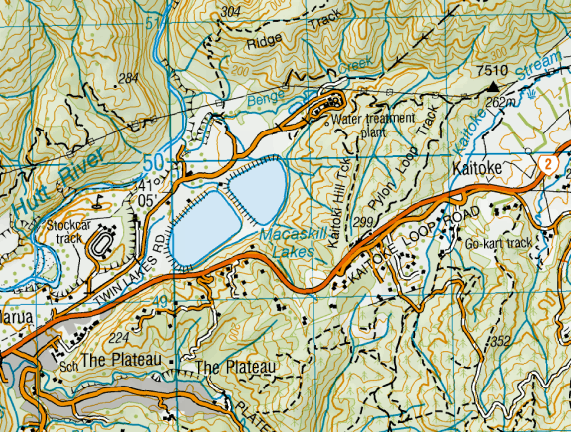
\includegraphics[width=0.45\textwidth]{lakes}
            \end{center}
    \end{enumerate}
  \end{exercise}

  \begin{exercise}
    In exercise \ref{ex:typesofquadrilaterals} we named several different types of quadrilaterals. Find the area of each.
  \end{exercise}

  \begin{exercise}
    Let $ ABC $ be a triangle; let $ D $ and $ E $ be points on $ [B,C] $. Then
    \begin{equation}
      \frac{\mathcal{A}(ABD)}{\mathcal{A}(ACE)} = \frac{\abs{BD}}{\abs{EC}}.
    \end{equation}
  \end{exercise}

  Using the theory of area we may prove the side-splitter theorem.

  \begin{prp}[Side-splitter theorem]\label{prp:sidesplitter}\index{Side-splitter theorem}
    Let $ ABC $ be a triangle and let $ \ell $ be a line parallel to $ \overline{BC} $ intersecting $ [A,B] $
    at $ D $ and $ [A,C] $ at $ E $. Then the following proportions hold:
    \begin{equation}\label{eqn:sidesplitter}
      \frac{\abs{AD}}{\abs{AB}} = \frac{AE}{AC} \text{ and } \frac{\abs{AD}}{\abs{DB}} = \frac{\abs{AE}}{\abs{EC}}.
    \end{equation}
  \end{prp}
  \begin{proof}
    \begin{multline*}
      \frac{\abs{AD}}{\abs{AB}} = \frac{\mathcal{A}(AED)}{\mathcal{A}(AEB)} = \frac{\mathcal{A}(AED)}{\mathcal{A}(AED) + \mathcal{A}(EBD)}\\
                                = \frac{\mathcal{A}(AED)}{\mathcal{A}(AED) + \mathcal{A}(ECD)} = \frac{\mathcal{A}(ADE)}{\mathcal{A}(ADC)} = \frac{\abs{AE}}{\abs{AC}}.
    \end{multline*}

    [Exercise: prove the second equality in (\ref{eqn:sidesplitter}).]
  \end{proof}

  \begin{exercise}\label{ex:ngonarea1}
    Find the area of a regular $ n$--gon with side length $ x $.

    Hints:
    \begin{itemize}
      \item There is a point inside the polygon which is equidistant from every vertex. You may assume this without proof. Try rearranging
            the triangles you can form using this point, and apply the previous exercise.
      \item You should get a slightly different answer for odd $ n $ than for even $ n $.
    \end{itemize}

    Compare with exercise \ref{ex:ngonarea2}
  \end{exercise}

  \begin{exercise}
    By utilising the same `approximation' trick as in exercise \ref{ex:circumference}, show that the area
    of a circle of radius $ r $ is $ \pi r^2 $.
  \end{exercise}

  \begin{exercise}\label{ex:pilowerbound}
    Compare with exercise \ref{ex:piupperbound}.
    Draw a circle of radius 1; pick four equally spaced points $ A $, $ B $, $ C $, $ D $ on the circumference, forming a square within
    the circle. Let $ O $ be the centre of the circle; then (prove all these statements) the four angles at $ O $ are right angles;
    thus the area of the square is the sum of areas of four triangles with bases 1 and heights 1; hence $ \pi > 2 $.
  \end{exercise}

  \chapter{Trigonometry}
  A \df{right-angled triangle} is, as the name suggests, a triangle with a right angle. The side of the triangle
  opposite the right angle is called the \df{hypotenuse}, and the other two sides are called the \df{legs}.

  \section{Pythagoras' theorem}
  The main goal of this section is to present a number of proofs of the following well-known theorem.
  \begin{thm}[Pythagoras]\index{Pythagoras' theorem}
    Let us consider a right-angled triangle with leg lengths $ a $ and $ b $, and hypotenuse length $ c $. Then
    \begin{equation}
      a^2 + b^2 = c^2.
    \end{equation}

    Equivalently, the area of the square on the hypotenuse is equal to the sum of the areas of the squares on the two other sides.
  \end{thm}

  Pythagoras was a Greek philosopher active in the middle of the 6th century BCE; it is likely that he was born on the island
  of Samos in the Aegean sea --- this is at least according to Ovid, \autocite[book XV, from line 60]{ovid} --- and his followers,
  the Pythagoreans, were a rather strange religous sect. See \autocite[58-60]{kline} for a lighthearted discussion of the Pythagoreans.

  It is believed that the theorem was also known by the ancient Egyptian, Indian, and Chinese civilisations (although it is unknown whether
  they had deductive proofs in the same sense as the Greeks).

  The Pythagoran theorem is useful because it allows us to find distances between two points if we know the horizontal and vertical
  distances between them. This in turn allows us to assign coordinates to points in the normal (Cartesian) way, with no
  problems.

  \subsection*{Applications and consequences of Pythagoras' theorem}
  \begin{exercise}\leavevmode
    \begin{enumerate}
      \item A rectangle has side lengths 3 and 4. What is the length of the diagonal?
      \item A rectangle has diagonal length 13 and one side length 5. What is the length of the remaining side?
      \item A rectangular box has side lengths 2, 3, 7. What is the longest stick that fits in the box?
      \item Show that the two diagonals of a rectangle are the same length.
      \item A right triangle has leg lengths in the ratio $ 3:5 $ and area 20. How long is the hypotenuse?
      \item A ship travels \SI{5}{\kilo\metre} south, \SI{2}{\kilo\metre} east, \SI{1}{\kilo\metre} north,
            and \SI{6}{\kilo\metre} west. How far away is it from its starting point as the crow flies?
      \item Let $ ABCD $ be a normal quadrilateral such that the internal angles at $ A $ and $ B $ are
            right angles. Find the length $ \abs{AB} $ if the opposite edge has length 20 and the two adjacent
            sides have lengths of 8 and 12.
    \end{enumerate}
  \end{exercise}

  \begin{exercise}\leavevmode
    \begin{enumerate}
      \item A square has area $ A $. What is the length of its diagonal?
      \item A rectangle has area $ A $. Do you have enough information to find the length of its diagonal?
            If so, find the diagonal length. If not, what other information might you need?
    \end{enumerate}
  \end{exercise}

  \begin{exercise}
    Suppose a right triangle has leg lengths $ 8 $ and $ 15 $.
    \begin{enumerate}
      \item Find the length of the hypotenuse.
      \item What happens to the length of the hypotenuse if:
        \begin{itemize}
          \item Both the leg lengths are doubled?
          \item Both the leg lengths are tripled?
          \item Both the leg lengths are multiplied by a number $ \mu $?
        \end{itemize}
    \end{enumerate}
  \end{exercise}

  \begin{exercise}
    Let $ ABC $ be a right triangle with right angle at $ C $. What is the relationship between the
    areas of the semicircles with diameter $ \abs{AB} $, $ \abs{AC} $, and $ \abs{BC} $?
  \end{exercise}

  \begin{exercise}
    Recall that an \df{integer} is a number of the form $ ..., -2, -1, 0, 1, 2, ... $.

    A \df{rational number} is a number which can be written in the form $ a/b $, where $ a $ and $ b $ are
    integers. The question is, are all numbers rational? (Clearly all integers are rational: if $ z $ is an integer, then $ z = z/1 $
    and 1 is an integer.)

    It turns out that the answer is no, and one simple example of an \df{irrational} number is the hypotenuse of the right-angled
    triangle with side length 1: $ \sqrt{1^2 + 1^2} = \sqrt{2} $.

    The (undoubtably false, though often repeated) story goes that the Pythagoreans were so upset at this result --- and the
    loss of their philosophy that all nature reduced to whole numbers or fractions --- that they threw the discoverer off
    a boat and into the sea, and vowed never to reveal the discovery. (See \autocite[\S4-3]{kline}.)

    \begin{enumerate}
      \item Justify why every rational number can be written in the form $ a/b $ where one of $ a $ or $ b $ is odd.
      \item Show that if $ a $ is an integer, then $ a^2 $ is odd exactly when $ a $ is odd and $ a^2 $ is even
            exactly when $ a $ is even.
      \item Suppose $ \sqrt{2} = a/b $, where $ a $ and $ b $ are integers. Suppose we have written it in the form
            of (1); that is, either $ a $ or $ b $ (or both) is odd. Show that $ a^2 = 2b^2 $.
      \item Using the previous result, show that $ a $ is even. Hence $ a = 2a' $ for some integer $ a' $.
      \item Thus $ (2a')^2 = 2b^2 $.
      \item Thus $ b^2  = 2a'^2 $, and hence $ b $ is even.
      \item Use (4) and (6) to arrive at an absurdity.
    \end{enumerate}
  \end{exercise}

  \begin{exercise}
    Let $ ABC $ be a triangle, and let $ D $ be the foot of the altitude from $ A $ onto $ BC $. Show
    that, if $ E $ is any point on $ [A,D] $, then
    \begin{equation}
      \abs{AC}^2 - \abs{CE}^2 = \abs{AB}^2 - \abs{EB}^2.
    \end{equation}

    What if:
    \begin{enumerate}
      \item $ E $ lies on the ray $ \ray{AD} $?
      \item $ E $ lies on the ray $ \ray{DA} $?
    \end{enumerate}
    \autocite[problem 3-1]{challenging}
  \end{exercise}

  \subsection*{Proofs of Pythagoras' theorem}
  \begin{exercise}[An area pushing proof]
    Suppose $ a $, $ b $, and $ c $ are sides of a right angled triangle as specified
    in the theorem statement.

    Let $ ABCD $ be a square of side length $ a + b $ such that each side is divided
    into segments of length $ a $ and length $ b $, and the division alternates around
    the square. Call the points of division $ E $, $ F $, $ G $, $ H $ so that $ E $
    is on the segment $ [A,B] $, $ F $ is on $ [B,C] $, $ G $ is in $ [C,D] $, and $ H $
    is on $ [D,A] $.

    \begin{enumerate}
      \item Show that $ EFGH $ is a square of side length $ c $.
      \item Thus the area of the square $ ABCD $ can be written as the sum of the areas
            of four right-angled triangles and the area of $ EFGH $. Do so.
      \item But the area can also be written as $ (x + y)^2 $. Set these two different expressions for the area equal to each other.
      \item Prove Pythagoras' theorem.
    \end{enumerate}
  \end{exercise}

  \begin{exercise}[A proof via similar triangles]
    Let $ ABC $ be a triangle with right angle at $ C $, hypotenuse length $ c $, and leg lengths $ a $ (opposite $ A $) and $ b $
    (opposite $ B $). Let $ H $ be the foot of the altitude of $ ABC $ from $ C $ to $ \overline{AB} $. Let $ \alpha $ be the measure
    of the angle at $ A $ and $ \beta $ be the measure of the angle at $ B $. Let $ x = \abs{BH} $ so $ c - x = \abs{AH} $.

    \begin{enumerate}
      \item Show that $ ABC \sim ACH $ and $ ABC \sim CBH $.
      \item Conclude that $ \frac{b}{c - x} = \frac{c}{b} $ and $ \frac{a}{x} = \frac{c}{a} $.
      \item Prove Pythagoras' theorem.
    \end{enumerate}
  \end{exercise}

  For Euclid's proof via area dissection, see Theorem 1.2 of my L3 trigonometry notes \autocite{myTrig}.

  For a proof via the `power of a point with respect to a circle', see exercise \ref{ex:pythviapower}.

  A large collection of other proofs can be found in \autocite{pythag}.

  \section{Triangle ratios}
  \begin{prp}
    Let a right angled triangle have side lengths $ a $, $ o $, and $ h $, where $ h $ is the length of the hypotenuse. Then the ratios $ o/h $, $ a/h $,
    and $ o/a $ depend only on the angle $ \theta $ at the vertex opposite $ o $.
  \end{prp}
  \begin{proof}
    This is a special case of exercise \ref{ex:similar}.3.
  \end{proof}

  Because the angles depend only on $ \theta $, we need only specify $ \theta $ to identify them. We call the length $ a $ the \df{adjacent leg},
  and the length $ o $ the \df{opposite leg}. We then defined the \df{sine}, \df{cosine}, and \df{tangent} functions by
  \begin{gather}
    \sin \theta = \frac{o}{h} = \frac{\text{opposite}}{\text{hypotenuse}},\\
    \cos \theta = \frac{a}{h} = \frac{\text{adjacent}}{\text{hypotenuse}},\text{ and}\\
    \tan \theta = \frac{o}{a} = \frac{\text{opposite}}{\text{adjacent}}.
  \end{gather}
  Together these three functions are called the \df{trigonometric functions}.

  \begin{exercise}[Finding lengths of triangles]
    The majority of these (purely computational) problems are taken from \autocite{foerster}.
    \begin{enumerate}
      \item Draw (accurately) a right angled triangle with one leg \SI{8}{\centi\metre} long
            and one acute angle of measure \ang{34} with the \SI{8}{\centi\metre} leg as its adjacent
            side. Calculate the lengths of the other leg and the hypotenuse using the relevant trigonometric functions;
            use a ruler to measure the lengths and check your results agree to within one millimetre.
      \item You must order a new rope for a flagpole. To find out what length of rope you need, you observe that the pole
            casts a shadow of \SI{11.6}{\metre} long on the ground. The angle of elevation of the sun is \ang{36;50;0}. How
            tall is the pole?
      \item A cat is trapped on a tree branch \SI{6.5}{\metre} above the ground. Your ladder is only \SI{6.7}{\metre} long.
            If the very end of the ladder is leant on the branch, what angle will the ladder make with the ground?
      \item Air New Zealand's domestic jet flights travel at a maximum altitude of around \SI{8000}{\metre}. They start
            descending when they are quite far away from the airport, so that they will not have to dive at a steep angle.
        \begin{enumerate}
          \item If the pilot wants the plane's path to make an angle of \ang{3} with the ground, how far away from the destination
                airport must they start descending?
          \item If the pilot begins a descent \SI{150}{\kilo\metre} away, what angle will the plane's path make with the horizontal?
          \item Generally, jet flights travel at around \SI{10000}{\metre} above the ground: an extra \SI{2}{\kilo\metre} above the
                height travelled by domestic flights in New Zealand. Why do you think domestic flights here travel lower than might
                be expected (especially as planes are often more fuel-efficient at their normal height of ten kilometres)? (Useful
                fact: the distance between Wellington and Christchurch airports is approximately \SI{300}{\kilo\metre}).
        \end{enumerate}
      \item Baldwin Street in Dunedin is often cited as the `steepest street in the world' (for example, by Guinness World Records).
            It has a slope of \ang{19}; if you walk along the street so you have travelled one metre horizontally, how far have you
            travelled vertically? How far do you have to travel horizontally in order to rise by one metre?
      \item The James Webb Space Telescope, the replacement for the Hubble Telescope due to launch in 2021, has a resolution of \ang{0;0;0.32} ---
            when the lines drawn between two stars and the telescope make this angle or greater, then it will be able to distinguish between them.\footnote{\textit{Tweet Chat with John Mather} (James Webb Space Telescope project scientist), retrieved from \url{https://jwst.nasa.gov/faq_tweetchat1.html} on 21 May 2019.}

            One light year is the distance that a beam of light will travel in one earth year; it is \SI{9.461e15}{\metre}.
        \begin{enumerate}
          \item Alpha Centauri, the closest star system to the Sun, is actually made up of three stars orbiting each other (named Rigil Kentaurus,
                Toliman, and Proxima Centauri). The naked eye sees one single blob of light. The distance between the stars is approximately \SI{0.21}{\lightyear},
                and the system lies around \SI{4.37}{\lightyear} away from the Sun. Will the telescope see three seperate stars, or one blob of light?
          \item How far apart do two stars in the Andromeda Galaxy (2.537 million light years away) need to be for the telescope to be able to
                distingush between them? Given that the Andromeda Galaxy is roughly circular and has a radius of \SI{110000}{\lightyear},
                will the telescope be able to distinguish between \emph{any} stars in that galaxy?
        \end{enumerate}
    \end{enumerate}
  \end{exercise}

  \begin{exercise}
    Design and construct a piece of equipment to allow you to measure the angle of elevation of a tall structure (i.e. the
    angle made between the horizontal ground and the line joining the point of observation to the top of the building). Use
    your device to measure the height of a building.
  \end{exercise}

  \begin{exercise}
    Research how trigonometry can be used to measure areas and create maps. Some possible search terms could include:
    \begin{itemize}
      \item Theodolite
      \item Triangulation station
      \item Great Indian trigonometric survey
    \end{itemize}
  \end{exercise}

  \begin{exercise}[Finding more lengths and areas]
    The majority of these (purely computational) problems are taken from \autocite{kutepov}.
    \begin{enumerate}
      \item How long will a  (taut) transmission belt need to be when the two pulleys are \SI{12}{\centi\metre} and \SI{34}{\centi\metre}
            in diameter and their centres are one metre apart?
      \item Two points $ A $ and $ B $ lie on opposite sides of a road. In order to get from $ A $ to $ B $ it is necessary to
            drive \SI{3.5}{\kilo\metre} along a side road that joins the main road at an angle of \ang{40}, then drive \SI{2.5}{\kilo\metre}
            along the main road and turn right onto another side road which makes an angle \ang{70} with the main road, and drive
            another \SI{4}{\kilo\metre}. All sections of roads traversed are straight. By how much will the distance from $ A $ to $ B $
            be shortened if a straight road is built between them?
            \begin{center}
              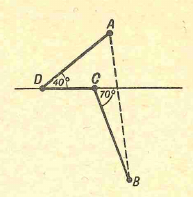
\includegraphics[width=0.5\textwidth]{roads}
            \end{center}
      \item At 7 o'clock in the morning a passenger plane took off from a town $ A $ and after thirty minutes stay in the town $ B $
            it took off again at 8.10, turned \ang{35} to the right, and landed in town $ C $ at 9.00. Determine the distance as-the-crow-flies
            between towns $ A $ and $ C $ if the average speed of the plane was \SI{320}{\kilo\metre\per\hour}.
      \item Two sides of a triangle are equal to \SI{5}{\centi\metre} and \SI{6}{\centi\metre}, and its area to \SI{5.28}{\centi\metre\squared}.
            Find the third side.
    \end{enumerate}
  \end{exercise}

  \begin{exercise}\leavevmode
    \begin{enumerate}
      \item A circle has circumference \SI{25.12}{\metre}. What is the area of the largest equilateral triangle that can be drawn in the circle?
      \item A circle has circumference $ C $. What is the area of the largest equilateral triangle that can be drawn in the circle?
    \end{enumerate}
  \end{exercise}

  \begin{exercise}\label{ex:ngonarea2}
    Find the area of a regular $ n$--gon $ \mathscr{P} $ with side length $ x $ by taking the centre of the polygon (you may assume
    that the centre --- a point equidistant from each vertex --- exists), cutting the polygon into $ 2n $ right angled
    triangles, and finding the area of each of these.

    You should find that
    \begin{equation}
      \mathcal{A}(\mathscr{P}) = \frac{x^2}{4\tan \frac{\ang{180}}{n}}.
    \end{equation}

    Compare this with exercise \ref{ex:ngonarea1}.
  \end{exercise}

  \chapter{Tilings and wallpaper patterns}
  Early in our studies we defined the concept of a \df{transformation}: a way of moving points around. We defined a \df{isometry}
  to be a transformation that preserved distance, and theorem \ref{thm:classisom} told us that there were only five kinds.

  \section{Symmetries}
  We call a figure \df{symmetric} if there is an isometry that transforms the figure to itself. If we can draw a line through
  a figure such that reflection through the line leaves the figure unchanged, then the line is called a \df{line of symmetry}.

  \begin{exercise}
    Find lines of symmetry for all the capital letters:

    \begin{center}
      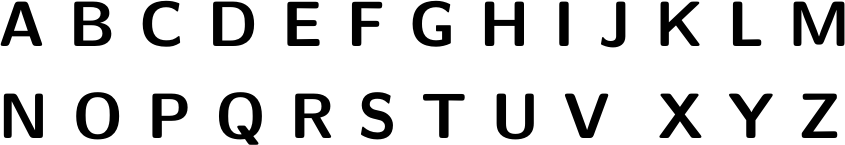
\includegraphics[width=\textwidth]{alphabet}
    \end{center}

    How many letters have no lines of symmetry? Which has the most?
  \end{exercise}

  \begin{exercise}
    The word BEE is made up of letters which are symmetric, and the word itself has
    a line of symmetry (horizontally through the middle). The word MUM has a vertical
    line of symmetry through the middle. Explain the differences between BEE, MUM, TOO, and EYE:
    all three are made up of symmetric letters, but not all have the same symmetries as words.
  \end{exercise}

  \begin{exercise}
    A figure is said to have a \df{centre of symmetry} $ O $ if we can rotate the figure around the
    point $ O $ by some angle (less than a full turn) so that the figure seems unchanged.

    Which letters have centres of symmetry, and through which angles can we rotate them?
  \end{exercise}

  Imagine that the following sequence of letters goes on to infinity in both
  directions.
  \begin{center}
    
\includegraphics[width=\textwidth]{translational}
  \end{center}

  If we translate the image left or right by a length which is a multiple of the distance
  between K's then the image appears unchanged. This is an example of a \df{translational
  symmetry}.

  \chapter{Circle inversion}
  Reflection is an important transformation in geometry; but why do we limit ourselves
  to reflection across lines?

  \section{The power of a circle}
  \begin{exercise}\label{ex:pythviapower}
    Suppose $ \mathscr{C} $ is a circle.
    \begin{enumerate}
      \item Suppose $ A $, $ B $, $ C $, and $ D $ are points on $ \mathscr{C} $ that form a normal
            quadrilateral $ ABCD $. Show that the opposite internal angles of $ ABCD $ add to \ang{180}.
      \item Suppose $ P $ is a point outside the circle, and let $ \ell $ and $ m $ be any two lines
            through $ P $ that intersect $ \mathscr{C} $ at $ A_\ell $ and $ B_\ell $, and $ A_m $ and $ B_m $
            respectively. Show that $ \abs{P A_\ell} \abs{P B_\ell} = \abs{P A_m} \abs{P B_m} $. So this
            quantity is independent of which line we choose: it only depends on $ P $ and $ \mathscr{C} $. This
            quantity is called the \df{power of the point} $ P $ with respect to $\mathscr{C} $, and we
            will write $ \mathrm{Pow}_\mathscr{C} P $ for this number.
      \item Let $ r $ be the radius of $ \mathscr{C} $, and let $ O $ be its centre. Pick a line through $ P $ that intersects the circle at
            a single point $ T $, and pick the point of the circle $ X $ that lies on $ [P,O] $; let $ d = \abs{PX} $. Show that
            $ \abs{PT}^2 = d^2 - r^2 $.
      \item Prove Pythagoras' theorem. \index{Pythagoras' theorem}
    \end{enumerate}
    See \autocite[14-15]{sved}.
  \end{exercise}

  \chapter{Spirals}

  \chapter{Three-dimensional geometry}

  \restoregeometry

  \clearpage
  \addcontentsline{toc}{chapter}{Bibliography and further reading}
  \printbibliography[title={Bibliography and further reading}]

  \clearpage
  \addcontentsline{toc}{chapter}{Index}
  \printindex

\end{document}
